% !TeX spellcheck = pl_PL

\rozdzial

%%%%%%%%%%%%%%%%%%%%%%%%%%%%%%%%%%%%%%%%%%%%%%%%%%%%%%%%%%%%%%%%%%%%%%%
\section{Wzorcowanie}
\label{wzorcowanie}

Do części związanej z wzorcowaniem przyrządów dozymetrycznych możemy przejść na dwa sposoby: z menu głównego (rys. \ref{menuGlowne}) lub z karty przyjęcia poprzez wciśnięcie przycisku \textbf{"Wzorcuj"} (patrz \ref{karta_przyjecia}). Jeżeli do części \textbf{"Wzorcowanie"} przechodzimy z menu głównego (patrz rozdz. \ref{menuGlowne}) program otwiera się na ostatniej karcie wpisanej w bazie danych. W przypadku przejścia za pomocą przycisku \textbf{"Wzorcuj"} z \textbf{"Karty przyjęcia"} (patrz rozdz. \ref{karta_przyjecia}) program podaje dane dla tej konkretnej karty.

Po lewej stronie okna \textbf{"Wzorcowanie"} program automatycznie podaje wprowadzone wcześniej w części \textbf{"Biuro"} (patrz rozdz. \ref{biuro}) informacje dla danej karty przyjęcia. Podane są: numer zlecenia do którego przypisana jest dana karta (pole \textbf{"Nr~zlecenia"}), nazwa zleceniodawcy (pole \textbf{"Zleceniodawca"}) oraz typ i numer fabryczny przyrządu (odpowiednio pola \textbf{"Typ"} i \textbf{"Numer fabryczny"}). 

\begin{figure}[htb]
	\centering
	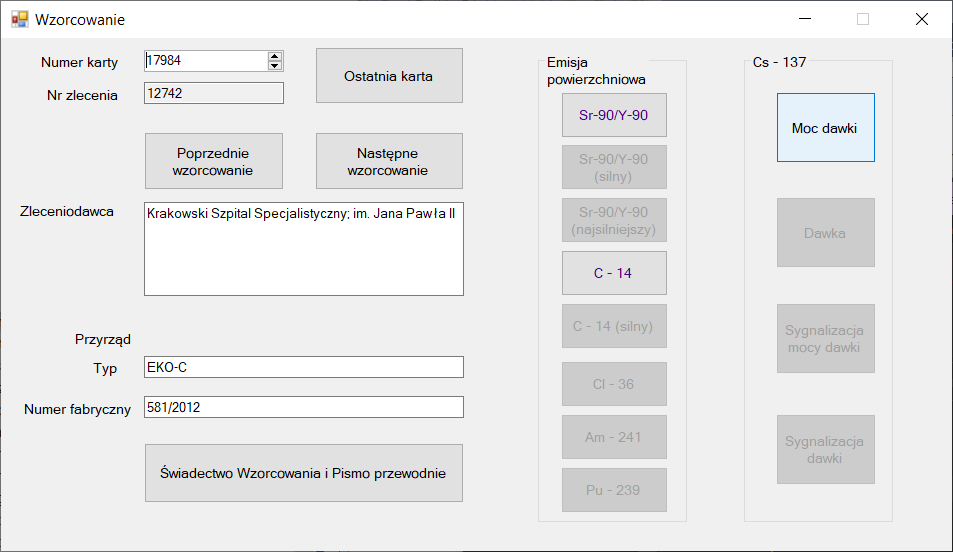
\includegraphics[width=\columnwidth]{obrazki/Wzorcowanie/menu_wzorcowanie.png}
	\caption{Główne okno wzorcowania}
	\label{menuWzorcowanie}
\end{figure}

Pomiędzy poszczególnymi numerami kart można się poruszać albo za pomocą trójkątów przy polu \textbf{"Numer karty"} albo poprzez ręczne wpisanie interesującego nas numeru karty.

Przyciski \textbf{"Poprzednie wzorcowanie"} i \textbf{"Następne wzorcowanie"} przenoszą nas automatycznie odpowiednio do poprzedniego lub następnego wzorcowania danego przyrządu (jeżeli takie istnieją).

Wciśnięcie przycisku \textbf{"Ostatnia karta"} powoduje przejście do ostatniego istniejącego w bazie danych numeru karty.

Znajdujący się na dole przycisk \textbf{"Świadectwo Wzorcowania i Pismo przewodnie"} powoduje przejście do modułu związanego z przygotowaniem i~wydrukiem Świadectwa Wzorcowania i Pisma przewodniego (patrz rozdz. \ref{swiadectwo_pismo}).

Po prawej stronie okna \ref{menuWzorcowanie} znajdują się przyciski pozwalające otworzyć okna związane z konkretnym typem wzorcowania. Dla Cs-137 są to moc dawki, dawka, sygnalizacja mocy dawki i sygnalizacja dawki. W zakresie emisji powierzchniowej dostępne jest każde z ośmiu źródeł. Dostępność przycisków zależy od zakresu wzorcowania wybranego w procesie wprowadzania karty przyjęcia (patrz rozdz. \ref{karta_przyjecia}).

\subsection{Wzorcowanie w zakresie mocy dawki}
\label{wzorcowanie_moc_dawki}

W górnej części okna znajdują się automatycznie wypełnione przez program pola \textbf{"Numer karty"}, \textbf{"Arkusz"} oraz \textbf{"Data"}. 

\textbf{TIP:} Za datę wzorcowania program domyślnie przyjmuję datę dzisiejszą, dlatego warto wprowadzać wyniki w dniu pomiaru. Jeżeli wprowadzamy wyniki wzorcowania przeprowadzonego wcześniej, należy pamiętać o zmianie tej daty na tę odpowiadającą pomiarom.

Po prawej stronie znajdują się przyciski \textbf{"Poprzedni arkusz"} i \textbf{"Następny arkusz"} umożliwiające poruszanie się pomiędzy poszczególnymi arkuszami pomiarowymi, jeżeli w tym zakresie istnieje więcej niż jeden arkusz (np. wykonujemy pomiary różnymi sondami, lub przy różnych ustawieniach przyrządu).

Przycisk \textbf{"Dane wzorcowe"} wyświetla dane wzorcowe przeliczone na daną datę i~jednostkę.

\textbf{TIP:} Z przycisku \textbf{"Dane wzorcowe"} warto skorzystać np. w celu ustalenia, w~którym punkcie i przy jakim źródle rozpocząć wzorcowanie.

W menu rozwijanym na górze okna znajdują się przyciski umożliwiające podgląd i~wydruk dokumentów (w tym przypadku protokołu kalibracyjnego mocy dawki oraz wykresu kalibracyjnego w zakresie mocy dawki) - \textbf{"Dokumenty"}. Obok jest przycisk \textbf{"Zapisz"}, który umożliwia zapisanie w bazie danych częściowo wprowadzonych wyników (jeżeli minimalne wymagania są spełnione - tzn. wybrany został typ i numer fabryczny sondy).

\begin{figure}[htb]
	\centering
	\includegraphics[width=\columnwidth]{obrazki/Wzorcowanie/moc_dawki/przyrzad.png}
	\caption{Okno wzorcowania w zakresie mocy dawki - zakładka przyrząd.}
	\label{mocPrzyrzad}
\end{figure}

W zakładce \textbf{"Przyrząd"} (rys. \ref{mocPrzyrzad}) znajdują się wszystkie dane dotyczące wzorcowanego przyrządu. Pola \textbf{"Typ"} oraz \textbf{"Numer fabryczny"} sekcji \textbf{"Przyrząd"} wypełniają się automatycznie danymi wprowadzonymi wcześniej dla danej karty przyjęcia. Poniżej znajduje się pole \textbf{"Inne nastawy przyrządu"}, do którego należy wprowadzić wszelkie dodatkowe informacje o ustawieniach, które mogą mieć wpływ na działanie przyrządu (np. stała czasowa, czułość wejścia itp.). Domyślnie pole to przyjmuje wartość "nie dotyczy".
	
W sekcji \textbf{"Sonda"} należy wypełnić pole \textbf{"Typ"} oraz \textbf{"Numer fabryczny"} sondy. Jeżeli mamy możliwość ustawienia napięcia zasilania sondy, to należy je wpisać w pole \textbf{"Napięcie zasilania sondy"}, w przeciwnym wypadku w polu pozostanie wartość domyślna "nie dotyczy".

\textbf{Ważne:} Należy zwrócić szczególną uwagę na wybór sondy w przypadku przyrządów, które posiadają więcej niż jedną sondę.

W zakładce \textbf{"Warunki"} (rys. \ref{mocWarunki}) przechowywane są informacje o warunkach w~jakich odbywało się wzorcowanie. W poszczególnych polach należy podać warunki atmosferyczne sczytane z termohigrobarometru: ciśnienie w hektopaskalach (pole \textbf{"Ciśnienie"}), temperaturę w stopniach Celsjusza (pole \textbf{"Temperatura"}) oraz wilgotność w procentach (pole \textbf{"Wilgotność"}).

\textbf{TIP:} Zgodnie z procedurą wzorcowanie można przeprowadzać jedynie jeżeli warunki atmosferyczne mieszczą się w następujących granicach: temperatura 15-30 \textcelsius, ciśnienie 900-1060 hPa,  wilgotność względna 10\%-85\%. Jeżeli podane przez użytkownika wartości nie mieszczą się w podanych przedziałach, to pole w którym nastąpiło wyjście poza zakres podświetlone zostanie na pomarańczowo.


\begin{figure}[htb]
	\centering
	\includegraphics[width=\columnwidth]{obrazki/Wzorcowanie/moc_dawki/warunki.png}
	\caption{Okno wzorcowania w zakresie mocy dawki - zakładka warunki.}
	\label{mocWarunki}
\end{figure}

Pozostałe ważne dla wzorcowania informacje należy uzupełnić w polu \textbf{"Uwagi"}. Jeżeli przyrząd był wcześniej wzorcowany w Laboratorium Wzorcowania, program automatycznie wpisuje tutaj informację o numerze poprzedniego świadectwa. W tym polu podaje się również takie informacje jak np. czy sygnalizacja przekroczenia zakresu uruchamia się prawidłowo. 

\textbf{Ważne:} W przypadku przyrządów uszkodzonych, w polu \textbf{"Uwagi"} podaje się wszystkie informacje o rodzaju uszkodzenia (np. przyrząd się nie uruchamia, przyrząd nie reaguje na promieniowanie, przyrząd pokazuje to samo wskazanie bez względu na wielkość pola promieniowania, etc.). Jeżeli jest taka potrzeba, to przy zapisywaniu uwagi można stosować dowolne znaczniki języka HTML.

Poniżej znajduje się pole wyboru \textbf{"Przedłużona ważność wzorcowania"}, które należy zaznaczyć, jeżeli przyrząd posiada przedłużoną ważność wzorcowania. Standardowo ważność wzorcowania wynosi rok, jednak w przypadku przyrządów posiadających własne źródło kontrolne ważność ta może zostać przedłużona do dwóch lat.

\begin{figure}[htb]
	\centering
	\includegraphics[width=\columnwidth]{obrazki/Wzorcowanie/moc_dawki/dane.png}
	\caption{Okno wzorcowania w zakresie mocy dawki - zakładka dane wzorcowe i pomiarowe.}
	\label{mocDane}
\end{figure}

Kolejna zakładka to \textbf{"Dane wzorcowe i pomiarowe"} (rys. \ref{mocDane}). To tutaj wprowadza się wyniki wzorcowania. Najpierw należy wybrać używany protokół kalibracyjny ławy (lista rozwijana \textbf{"Protokół"}), jednostkę (lista rozwijana \textbf{"Jednostka"}) oraz przypisaną do niej wielkość fizyczną (lista rozwijana \textbf{"Wielkość fizyczna"}). Dzięki tym informacjom i podanej wcześniej dacie wzorcowania program może przygotować wspomniane wcześniej dane wzorcowe (dostępne po kliknięciu przycisku \textbf{"Dane wzorcowe"}).

\textbf{TIP:} Najnowszy protokół kalibracyjny ławy znajduje się na samym dole listy rozwijanej \textbf{"Protokół"}.

\textbf{TIP:} Po wybraniu jednostki na liście rozwijanej \textbf{"Wielkość fizyczna"} pozostaje jedynie wielkość fizyczna przypisana do tej jednostki. Można jednak dowolnie ją zmienić wpisując inną wielkość fizyczną ręcznie.

Jako pierwszy wykonujemy pomiar tła. Otrzymaną wartość wpisujemy w polu \textbf{"Tło"}. Następnie szukamy punktu, w którym moc dawki jest jak najbardziej zbliżona do zakresu przyrządu (ale mniejsza od niego). Warto w tym celu posłużyć się danymi wzorcowymi. W tabeli wpisujemy odległość naświetlania (kolumna 1 - \textbf{"Odległość"}) oraz numer zastosowanego źródła (kolumna 2 - \textbf{"Źródło"}). Jako numer źródła wpisujemy: 1, 2 lub 3, gdzie 3 to źródło najsilniejsze, a 1 najsłabsze). W kolumnie piątej - \textbf{"Zakres"} podajemy zakres, dla którego wykonywany jest pomiar (w przypadku przyrządów z jednym zakresem, jest to cały czas ten sam zakres maksymalny).

Dostępne są dwie opcje wprowadzania wyników: jedna to bezpośrednie podanie wskazania i jego wahania w tabeli (kolumny \textbf{"Wskazanie"} i \textbf{"Niepewność"}), druga to podanie maksymalnej i minimalnej wartości wskazanej przez przyrząd (kolumny \textbf{"Min"} i \textbf{"Max"}). W drugim przypadku program automatycznie wyliczy wskazanie (jako średnią arytmetyczną wartości maksymalnej i minimalnej) oraz niepewność (jako różnicę wyliczonego wskazania i wartości minimalnej).

Aby program podał w tabeli wartości wzorcowe (kolumna \textbf{"Wartość wzorcowa"}) oraz (jeżeli to wymagane) wskazanie i wahanie (z \textbf{"Min"} i \textbf{"Max"}) należy wcisnąć przycisk \textbf{"Licz"}. 

\textbf{Ważne:} Jeżeli w danym wierszu tabeli \textbf{"Wartość wzorcowa"} nie zostanie wyświetlona należy sprawdzić podane w tym wierszu odległość i źródło. Brak wyświetlenia wartości wzorcowej oznacza bowiem, że w wybranym protokole nie ma danych wzorcowych dla takiej kombinacji odległość - źródło.

Jeśli nie ma jakichś szczególnych przesłanek, aby robić inaczej, to kolejne punkty ustalamy tak, aby były 3 punkty na każdy zakres pomiarowy (w przypadku przyrządów posiadających kilka krótszych zakresów pomiarowych), albo aby były co najmniej trzy punkty na dekadę (w przypadku przyrządów o długim zakresie).

\textbf{TIP:} W trakcie wzorcowania warto posłużyć się punktami użytymi podczas poprzedniego wzorcowania przyrządu (jeżeli istnieje). Z jednej strony bardzo przyspiesza to pracę, z drugiej łatwiej porównać potem oba wyniki i wykryć ewentualne różnice.

Przycisk \textbf{"Dołączyć wszystko"} automatycznie zaznacza wszystkie pola wyboru w~kolumnie \textbf{"Dołączyć"}. Kolumna ta wskazuje programowi, które punkty ma brać pod uwagę przy wyliczaniu współczynnika kalibracyjnego oraz jego niepewności. Zdarzają się przyrządy, które w górnej części swojego zakresu ulegają nasyceniu i ich odpowiedź nie jest już proporcjonalna do wielkości pola promieniowania. Wtedy zakres takiego przyrządu należy ograniczyć do liniowej części odpowiedzi. Drugim przypadkiem, w którym warto rozważyć odłączenie danego punktu, są punkty w niskich polach promieniowania, których wahanie jest bardzo duże - niewspółmierne do wahań przyrządu w średnich i wysokich polach promieniowania.

\begin{figure}[htb]
	\centering
	\includegraphics[width=\columnwidth]{obrazki/Wzorcowanie/moc_dawki/wspolczynniki.png}
	\caption{Okno wzorcowania w zakresie mocy dawki - zakładka obliczone współczynniki.}
	\label{mocWspolczynniki}
\end{figure}

W zakładce \textbf{"Obliczone współczynniki"} (rys. \ref{mocWspolczynniki}) znajdują się pola \textbf{"Wykonał(a)"} i \textbf{"Sprawdził(a)"}, w których należy podać odpowiednio osobę, która wykonywała wzorcowanie i osobę, która będzie wykonanie tego wzorcowania sprawdzać. 

\textbf{TIP:} Program zapamiętuje ostatnio wpisane dane i automatycznie uzupełnia te pola \textbf{"Wykonał(a)"} i \textbf{"Sprawdził(a)"} tymi danymi. Należy więc zwrócić na to szczególną uwagę przy zmianie pracownika wykonującego/sprawdzającego wzorcowanie.

Poniżej znajdują się pola wyboru: \textbf{"Dołączyć do świadectwa"} - domyślnie zaznaczone pole oznaczające, że wyniki z tego arkusza mają być zawarte w Świadectwie Wzorcowania oraz \textbf{"Poprawa"} - pole wyboru, które należy zaznaczyć jeżeli arkusz jest wynikiem korekty wcześniejszego wzorcowania (w wydrukach dokumentów numer karty będzie posiadał dodatkową literę \textbf{"P"}).

Przycisk \textbf{"Oblicz"} powoduje wyświetlenie w tabeli wyników wzorcowania dla każdego z zakresów przyrządu (kolumny \textbf{"Zakres"}, \textbf{"Współczynnik"} i~\textbf{"Niepewność"}). Jeżeli przyrząd był już wzorcowany w zakresie mocy dawki (i~w~danym zakresie pomiarowym przyrządu), to w dwóch ostatnich kolumnach tabeli (\textbf{"Poprzedni współczynnik"} i \textbf{"Poprzednia niepewność"}) pojawią się współczynnik i niepewność z poprzedniego wzorcowania. 

\textbf{TIP:} Warto zawsze porównać ze sobą oba wyniki wzorcowania, aby wychwycić ewentualne rozbieżności i spróbować znaleźć ich źródło (czy to błąd we wzorcowaniu, czy np. jakieś uszkodzenie przyrządu).

\textbf{Ważne:} Poza jednostkowymi wyjątkami (przyrządy typu RUST-2, RUST-3, RUM-1) dla większości typów przyrządów idealnym współczynnikiem jest współczynnik 1 z jak najmniejszą niepewnością. Co pokazuje, że wskazania przyrządu odpowiadają rzeczywistym wartościom pola promieniowania. Należy więc zwrócić szczególną uwagę na wyniki znacznie odbiegające od 1, lub z bardzo dużą niepewnością w stosunku do współczynnika. Takie wyniki mogą sugerować błąd we wzorcowaniu, lub wpisywaniu danych do programu, albo też niesprawność przyrządu. W ocenie poprawności wzorcowania pomaga także analiza wykresu kalibracyjnego.

Każdorazowo przy zamknięciu okna \textbf{"Wzorcowanie cezem - Moc Dawki"} program zapyta o to czy chcemy zapisać wprowadzone zmiany.

\subsection{Wzorcowanie w zakresie dawki}
\label{wzorcowanie_dawka}

W górnej części okna znajdują się automatycznie wypełnione przez program pola \textbf{"Numer karty"}, \textbf{"Arkusz"} oraz \textbf{"Data"}. 

\textbf{TIP:} Za datę wzorcowania program domyślnie przyjmuję datę dzisiejszą, dlatego warto wprowadzać wyniki w dniu pomiaru. Jeżeli wprowadzamy wyniki wzorcowania przeprowadzonego wcześniej, należy pamiętać o zmianie tej daty na tę odpowiadającą pomiarom.

Po prawej stronie znajdują się przyciski \textbf{"Poprzedni arkusz"} i \textbf{"Następny arkusz"} umożliwiające poruszanie się pomiędzy poszczególnymi arkuszami pomiarowymi, jeżeli w tym zakresie istnieje więcej niż jeden arkusz (np. wykonujemy pomiary różnymi sondami, lub przy różnych ustawieniach przyrządu).

Przycisk \textbf{"Dane wzorcowe"} wyświetla dane wzorcowe przeliczone na daną datę i~jednostkę.

\textbf{TIP:} Z przycisku \textbf{"Dane wzorcowe"} warto skorzystać np. w celu ustalenia, w~którym punkcie wykonywać naświetlanie przyrządu, jeżeli standardowo stosowana odległość 288,5 cm jest z jakichś przyczyn niedostępna.

\begin{figure}[htb]
	\centering
	\includegraphics[width=\columnwidth]{obrazki/Wzorcowanie/dawka/przyrzad.png}
	\caption{Okno wzorcowania w zakresie dawki - zakładka przyrząd.}
	\label{dawkaPrzyrzad}
\end{figure}

W menu rozwijanym na górze okna znajdują się przyciski umożliwiające podgląd i~wydruk dokumentów (w tym przypadku protokołu kalibracyjnego dawki oraz wykresu kalibracyjnego w zakresie dawki) - \textbf{"Dokumenty"}. Obok jest przycisk \textbf{"Zapisz"}, który umożliwia zapisanie w bazie danych częściowo wprowadzonych wyników (jeżeli minimalne wymagania są spełnione - tzn. wybrany został typ i snumer fabryczny sondy).

W zakładce \textbf{"Przyrząd"} (rys. \ref{dawkaPrzyrzad}) znajdują się wszystkie dane dotyczące wzorcowanego przyrządu. Pola \textbf{"Typ"} oraz \textbf{"Numer fabryczny"} sekcji \textbf{"Przyrząd"} wypełniają się automatycznie danymi wprowadzonymi wcześniej dla danej karty przyjęcia. Poniżej znajduje się pole \textbf{"Inne nastawy przyrządu"}, do którego należy wprowadzić wszelkie dodatkowe informacje o ustawieniach, które mogą mieć wpływ na działanie przyrządu. Domyślnie pole to przyjmuje wartość "nie dotyczy".

W sekcji \textbf{"Sonda"} należy wypełnić pole \textbf{"Typ"} oraz \textbf{"Numer fabryczny"} sondy. Jeżeli mamy możliwość ustawienia napięcia zasilania sondy, to należy je wpisać w pole \textbf{"Napięcie zasilania sondy"}, w przeciwnym wypadku w polu pozostanie wartość domyślna "nie dotyczy".

\textbf{Ważne:} Należy zwrócić szczególną uwagę na wybór sondy w przypadku przyrządów, które posiadają więcej niż jedną sondę.

\begin{figure}[htb]
	\centering
	\includegraphics[width=\columnwidth]{obrazki/Wzorcowanie/dawka/warunki.png}
	\caption{Okno wzorcowania w zakresie dawki - zakładka warunki.}
	\label{dawkaWarunki}
\end{figure}

W zakładce \textbf{"Warunki"} (rys. \ref{dawkaWarunki}) przechowywane są informacje o warunkach w~jakich odbywało się wzorcowanie. W poszczególnych polach należy podać warunki atmosferyczne sczytane z termohigrobarometru: ciśnienie w hektopaskalach (pole \textbf{"Ciśnienie"}), temperaturę w stopniach Celsjusza (pole \textbf{"Temperatura"}) oraz wilgotność w procentach (pole \textbf{"Wilgotność"}).

\textbf{TIP:} Zgodnie z procedurą wzorcowanie można przeprowadzać jedynie jeżeli warunki atmosferyczne mieszczą się w następujących granicach: temperatura 15-30 \textcelsius, ciśnienie 900-1060 hPa,  wilgotność względna 10\%-85\%. Jeżeli podane przez użytkownika wartości nie mieszczą się w podanych przedziałach, to pole w którym nastąpiło wyjście poza zakres podświetlone zostanie na pomarańczowo.

Pozostałe ważne dla wzorcowania informacje należy uzupełnić w polu \textbf{"Uwagi"}. Jeżeli przyrząd był wcześniej wzorcowany w Laboratorium Wzorcowania, program automatycznie wpisuje tutaj informację o numerze poprzedniego świadectwa. W tym polu podaje się również takie informacje jak np. czy sygnalizacja przekroczenia zakresu uruchamia się prawidłowo. 

\textbf{Ważne:} W przypadku przyrządów uszkodzonych, w polu \textbf{"Uwagi"} podaje się wszystkie informacje o rodzaju uszkodzenia (np. przyrząd się nie uruchamia, przyrząd nie reaguje na promieniowanie, przyrząd pokazuje to samo wskazanie bez względu na wielkość pola promieniowania, etc.). Jeżeli jest taka potrzeba, to przy zapisywaniu uwagi można stosować dowolne znaczniki języka HTML.

Kolejna zakładka to \textbf{"Dane wzorcowe i pomiarowe"} (rys. \ref{dawkaDane}). Tutaj wprowadza się wyniki wzorcowania. Najpierw należy wybrać używany protokół kalibracyjny ławy (lista rozwijana \textbf{"Protokół"}), wybrane źródło (pole \textbf{"Źródło"}) i odległość, na której przyrząd będzie naświetlany (pole \textbf{"Odległość"}). Źródła określone są numerami 1, 2 i 3, gdzie 1 to źródło o najmniejszej mocy dawki, a 3 o największej.

\textbf{TIP:} Najnowszy protokół kalibracyjny ławy znajduje się na samym dole listy rozwijanej \textbf{"Protokół"}.

Dodatkowo w polu \textbf{"Zakres"} wpisujemy zakres w jakim wzorcujemy. 

Na dole, po prawej stronie okna mamy możliwość wyboru jednej z czterech wielkości fizycznych:
\begin{itemize}
	\item indywidualnego równoważnika dawki $H_{p}(10)$;
	\item indywidualnego równoważnika dawki $H_{p}(0,07)$;
	\item indywidualnego równoważnika dawki $H^{*}$;
	\item mocy kermy.
\end{itemize}

\begin{figure}[htb]
	\centering
	\includegraphics[width=\columnwidth]{obrazki/Wzorcowanie/dawka/dane.png}
	\caption{Okno wzorcowania w zakresie dawki - zakładka dane wzorcowe i pomiarowe.}
	\label{dawkaDane}
\end{figure}

W pierwszej kolumnie tabeli (\textbf{"Wartość wzorcowa [mSv]"}) wpisujemy kolejne dawki jakimi zamierzamy naświetlać wzorcowany dawkomierz. Standardowo stosowane są dawki: 0,1; 0,2; 0,4; 0,8; 1,6; 3,2 oraz 6,4 mSv. Następnie wciskając znajdujący się po prawej stronie przycisk \textbf{"Licz"} otrzymujemy w tabeli w kolumnie \textbf{"Czas [s]"} czasy jakie są wymagane, aby dokonać ekspozycji przyrządu zadaną w kolumnie pierwszej dawką na wybranej wcześniej odległości i przy użyciu podanego źródła.

\textbf{Ważne:} Jeżeli czasy wyświetlone w tabeli wynoszą w każdym wierszu 0,00 s (bez względu na wielkość zadanej dawki) należy sprawdzić podane wcześniej odległość i źródło. Brak wyświetlenia sensownych czasów naświetlania oznacza bowiem, że w wybranym protokole nie ma danych wzorcowych dla takiej kombinacji odległość - źródło.

\textbf{Ważne:} Program zakłada, że kolejne dawki są sumowane, więc podaje czasy potrzebne do naświetlenia przyrządu dawką o wartości równej różnicy między dawką zadaną, a dawką poprzednią.

W trzeciej kolumnie (\textbf{"Wskazanie"}) wpisujemy wartości dawki w mSv wskazane po naświetleniu przez wzorcowany przyrząd.

Przycisk \textbf{"Dołącz wszystko"} automatycznie zaznacza wszystkie pola wyboru w~kolumnie \textbf{"Dołączyć"}. Kolumna ta wskazuje programowi, które punkty ma brać pod uwagę przy wyliczaniu współczynnika kalibracyjnego oraz jego niepewności.

\begin{figure}[htb]
	\centering
	\includegraphics[width=\columnwidth]{obrazki/Wzorcowanie/dawka/wspolczynniki.png}
	\caption{Okno wzorcowania w zakresie dawki - zakładka obliczone współczynniki.}
	\label{dawkaWspolczynniki}
\end{figure}

W zakładce \textbf{"Obliczone współczynniki"} (rys. \ref{dawkaWspolczynniki}) znajdują się pola \textbf{"Wykonał(a)"} i \textbf{"Sprawdził(a)"}, w których należy podać odpowiednio osobę, która wykonywała wzorcowanie i osobę, która będzie wykonanie tego wzorcowania sprawdzać. 

\textbf{TIP:} Program zapamiętuje ostatnio wpisane dane i automatycznie uzupełnia te pola \textbf{"Wykonał(a)"} i \textbf{"Sprawdził(a)"} tymi danymi. Należy więc zwrócić na to szczególną uwagę przy zmianie pracownika wykonującego/sprawdzającego wzorcowanie.

Poniżej znajduje się pole wyboru \textbf{"Dołączyć do świadectwa"} - domyślnie zaznaczone pole oznaczające, że wyniki z tego arkusza mają być zawarte w świadectwie wzorcowania.

Przycisk \textbf{"Oblicz"} powoduje wyświetlenie wyników wzorcowania w sekcji \textbf{"Wyniki wzorcowania"}, pola \textbf{"Współczynnik"} i~\textbf{"Niepewność"}). Jeżeli przyrząd był już wzorcowany w zakresie dawki, to w sekcji \textbf{"Wyniki poprzedniego wzorcowania"} w~polach \textbf{"Współczynnik"} i \textbf{"Niepewność"}) pojawią się odpowiednio współczynnik i~niepewność z poprzedniego wzorcowania. 

\textbf{TIP:} Warto zawsze porównać ze sobą oba wyniki wzorcowania, aby wychwycić ewentualne rozbieżności i spróbować znaleźć ich źródło (czy to błąd we wzorcowaniu, czy np. jakieś uszkodzenie przyrządu).

\textbf{Ważne:} Dla większości typów przyrządów idealnym współczynnikiem jest współczynnik 1 z jak najmniejszą niepewnością. Co pokazuje, że wskazania przyrządu odpowiadają rzeczywistym wartościom dawki jaką przyrząd był napromieniowany. Należy więc zwrócić szczególną uwagę na wyniki znacznie odbiegające od 1, lub z bardzo dużą niepewnością w stosunku do współczynnika. (Względne niepewności współczynnika kalibracyjnego w zakresie dawki są zazwyczaj rzędu kilku procent).s Takie wyniki mogą sugerować błąd we wzorcowaniu, lub wpisywaniu danych do programu, albo też niesprawność przyrządu. W ocenie poprawności wzorcowania pomaga także analiza wykresu kalibracyjnego.

Każdorazowo przy zamknięciu okna \textbf{"Wzorcowanie Dawki"} program zapyta o to czy chcemy zapisać wprowadzone zmiany.

\subsection{Wzorcowanie w zakresie sygnalizacji mocy dawki}
\label{wzorcowanie_syg_moc}

	W górnej części okna znajdują się wypełnione przez program pola \textbf{"Numer karty"}, \textbf{"Arkusz"} oraz \textbf{"Data"}. 
	
	\textbf{TIP:} Za datę wzorcowania program domyślnie przyjmuję datę dzisiejszą, dlatego warto wprowadzać wyniki w dniu pomiaru. Jeżeli wprowadzamy wyniki wzorcowania przeprowadzonego wcześniej, należy pamiętać o zmianie tej daty na tę odpowiadającą pomiarom.
	
	Po prawej stronie znajdują się przyciski \textbf{"Poprzedni arkusz"} i \textbf{"Następny arkusz"} umożliwiające poruszanie się pomiędzy poszczególnymi arkuszami, jeżeli w tym zakresie istnieje więcej niż jeden arkusz (np. wykonujemy pomiary różnymi sondami, lub przy różnych ustawieniach).
	
	Przycisk \textbf{"Dane wzorcowe"} wyświetla dane wzorcowe mocy dawki przeliczone na daną datę i jednostkę.
	
	\textbf{TIP:} Z przycisku \textbf{"Dane wzorcowe"} warto skorzystać np. w celu ustalenia na jakiej odległości i przy użyciu którego ze źródeł warto rozpocząć wzorcowanie. 
	
	W menu rozwijanym na górze okna znajdują się opcje umożliwiające podgląd i wydruk dokumentów (w tym przypadku protokołu kalibracyjnego sygnalizacji mocy dawki) - \textbf{"Dokumenty"} oraz przycisk \textbf{"Zapisz"}, który umożliwia zapisanie częściowych wyników (jeżeli minimalne wymagania są spełnione - wybrany został numer fabryczny sondy).
	
	\begin{figure}[H]
		\centering
		\includegraphics[width=\columnwidth]{obrazki/Wzorcowanie/syg_mocy_dawki/przyrzad.png}
		\caption{Okno wzorcowania w zakresie sygnalizacji mocy dawki - zakładka przyrząd.}
		\label{sygMocyPrzyrzad}
	\end{figure}
	
	W zakładce \textbf{"Przyrząd"} (rys. \ref{sygMocyPrzyrzad}) znajdują się wszystkie dane dotyczące wzorcowanego przyrządu. Pola \textbf{"Typ"} oraz \textbf{"Numer fabryczny"} sekcji \textbf{"Przyrząd"} wypełniają się automatycznie danymi wprowadzonymi dla danej karty przyjęcia. Poniżej znajduje się pole \textbf{"Inne nastawy przyrządu"}, do którego należy wprowadzić wszelkie dodatkowe informacje o ustawieniach które mogą mieć wpływ na działanie przyrządu. Domyślnie pole to przyjmuje wartość "nie dotyczy".
	
	W sekcji sonda należy wypełnić pole \textbf{"Typ"} oraz \textbf{"Numer fabryczny"} sondy. Jeżeli mamy możliwość ustawienia napięcia zasilania sondy, to należy je wpisać w pole \textbf{"Napięcie zasilania sondy"}, w przeciwnym wypadku pozostanie wartość domyślna "nie dotyczy".
	
	\textbf{TIP:} Należy zwrócić szczególną uwagę na wybór sondy w przypadku przyrządów, które posiadają więcej niż jedną sondę.
	
	\begin{figure}[htb]
	\centering
	\includegraphics[width=\columnwidth]{obrazki/Wzorcowanie/syg_mocy_dawki/warunki.png}
	\caption{Okno wzorcowania w zakresie sygnalizacji mocy dawki - zakładka warunki.}
	\label{sygMocyWarunki}
	\end{figure}
	
	W zakładce \textbf{"Warunki"} (rys. \ref{sygMocyWarunki}) przechowywane są informacje o warunkach w jakich odbywało się wzorcowanie. W poszczególnych polach należy podać warunki atmosferyczne sczytane z termohigrobarometru: ciśnienie, temperaturę oraz wilgotność.
	
	\textbf{TIP:} Zgodnie z procedurą wzorcowanie można przeprowadzać jedynie jeżeli warunki atmosferyczne mieszczą się w następujących granicach: temperatura 15-30 \textcelsius, ciśnienie 900-1060 hPa,  wilgotność względna 10\%-85\%. Jeżeli podane przez użytkownika wartości nie mieszczą się w podanych przedziałach, to pole w którym nastąpiło wyjście poza zakres podświetlone zostanie na pomarańczowo.
	
	Pozostałe ważne dla wzorcowania informacje należy uzupełnić w polu \textbf{"Uwagi"}. Jeżeli przyrząd był wcześniej wzorcowany w laboratorium, program automatycznie wpisuje informację o numerze poprzedniego świadectwa. 
	
	\textbf{TIP:} W przypadku przyrządów uszkodzonych, w polu \textbf{"Uwagi"} podaje się wszystkie informacje o rodzaju uszkodzenia (np. przyrząd się nie uruchamia, przyrząd nie reaguje na promieniowanie, przyrząd pokazuje to samo wskazanie bez względu na wielkość promieniowania, etc.).

	Kolejna zakładka to \textbf{"Dane wzorcowe i pomiarowe"} (rys. \ref{sygMocyDane}). Tutaj wprowadza się wyniki wzorcowania. Najpierw należy wybrać używany protokół kalibracyjny ławy (lista rozwijana \textbf{"Protokół"}) oraz jednostkę (lista rozwijana \textbf{"Jednostka"}).
	
	\textbf{TIP:} Najnowszy protokół kalibracyjny ławy znajduje się na samym dole listy rozwijanej \textbf{"Protokół"}.
	
	\begin{figure}[htb]
		\centering
		\includegraphics[width=\columnwidth]{obrazki/Wzorcowanie/syg_mocy_dawki/dane.png}
		\caption{Okno wzorcowania w zakresie sygnalizacji mocy dawki - zakładka dane wzorcowe i pomiarowe.}
		\label{sygMocyDane}
	\end{figure}
	


	Po prawej stronie mamy do wyboru dwie opcje uzupełniania wyników: \textbf{"Tabela"} lub \textbf{"Opis"}. Wybieramy jedną w zależności od wzorcowanego typu przyrządu. 
		
	W pierwszej kolumnie tabeli podajemy ustawiony na przyrządzie próg sygnalizacji mocy dawki. Naświetlanie przyrządu rozpoczynamy od punktu i źródła, przy których moc dawki jest niższa niż ustawiony próg. (W tym celu warto skorzystać z przycisku \textbf{"Dane wzorcowe"}). Następnie powoli przesuwamy się w kierunku wzrastających mocy dawek. W kolumnie drugiej (\textbf{"Odległość 1"}) i trzeciej (\textbf{"Nr źródła 1"}) podajemy odpowiednio odległość i numer źródła, przy których uruchomiła się sygnalizacja ostrzegawcza przyrządu. Następnie przesuwamy przyrząd w kierunku malejących mocy dawek i obserwujemy, kiedy nastąpi wyłączenie sygnalizacji ostrzegawczej. W kolumnach cztery (\textbf{"Odległość 2"}) i pięć (\textbf{"Nr źródła 2"}) podajemy odległość i numer źródła, przy których to nastąpiło. Następnie wciskając znajdujący się po prawej stronie przycisk \textbf{"Oblicz"} otrzymujemy w kolumnach od 6 do 9 odpowiednio wyliczoną rzeczywistą wartość, przy której uruchamia się sygnalizacja ostrzegawcza wraz z niepewnością oraz wyliczony na jej podstawie współczynnik kalibracyjny wraz z jego niepewnością.
	
		\begin{figure}[htb]
		\centering
		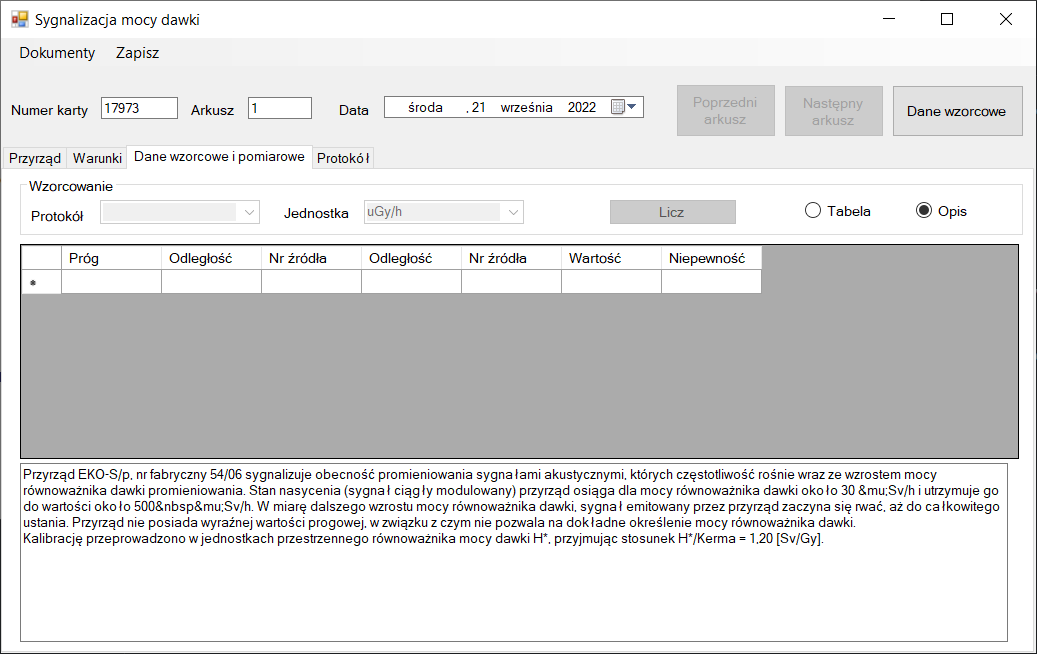
\includegraphics[width=\columnwidth]{obrazki/Wzorcowanie/syg_mocy_dawki/dane2.png}
		\caption{Okno wzorcowania w zakresie sygnalizacji mocy dawki - zakładka dane wzorcowe i pomiarowe.}
		\label{sygMocyDane2}
	\end{figure}

W przypadku opcji \textbf{"Opis"} (rys. \ref{sygMocyDane2}) wykonujemy opis zachowania przyrządu w polu promieniowania.
	
	\begin{figure}[htb]
		\centering
		\includegraphics[width=\columnwidth]{obrazki/Wzorcowanie/syg_mocy_dawki/wspolczynniki.png}
		\caption{Okno wzorcowania w zakresie sygnalizacji mocy dawki - zakładka obliczone współczynniki.}
		\label{sygMocyWspolczynniki}
	\end{figure}
	
	W zakładce \textbf{"Obliczone współczynniki"} (rys. \ref{sygMocyWspolczynniki}) znajdują się pola \textbf{"Wykonał(a)"} i \textbf{"Sprawdził(a)"}, w których należy podać odpowiednio dane osoby, która wykonywała wzorcowanie i osoby, która będzie to zatwierdzać. 
	
	\textbf{TIP:} Program zapamiętuje ostatnio wpisane dane i automatycznie uzupełnia te pola tymi danymi. Należy więc zwrócić na to szczególną uwagę przy zmianie pracownika wykonującego wzorcowanie.
	
	Poniżej znajduje się pole wyboru \textbf{"Dołącz do świadectwa"} - domyślnie zaznaczone pole oznaczające, że wyniki z tego arkusza mają być zawarte w świadectwie wzorcowania.

\subsection{Wzorcowanie w zakresie sygnalizacji dawki}
\label{wzorcowanie_syg_dawka}
	
	W górnej części okna znajdują się wypełnione przez program pola \textbf{"Numer karty"}, \textbf{"Arkusz"} oraz \textbf{"Data"}. 
	
	\textbf{TIP:} Za datę wzorcowania program domyślnie przyjmuję datę dzisiejszą, dlatego warto wprowadzać wyniki w dniu pomiaru. Jeżeli wprowadzamy wyniki wzorcowania przeprowadzonego wcześniej, należy pamiętać o zmianie tej daty na tę odpowiadającą pomiarom.
	
	\begin{figure}[htb]
		\centering
		\includegraphics[width=\columnwidth]{obrazki/Wzorcowanie/syg_dawki/przyrzad.png}
		\caption{Okno wzorcowania w zakresie sygnalizacji dawki - zakładka przyrząd.}
		\label{sygDawkiPrzyrzad}
	\end{figure}
	
	Po prawej stronie znajdują się przyciski \textbf{"Poprzedni arkusz"} i \textbf{"Następny arkusz"} umożliwiające poruszanie się pomiędzy poszczególnymi arkuszami, jeżeli w tym zakresie istnieje więcej niż jeden arkusz (np. wykonujemy pomiary różnymi sondami, lub przy różnych ustawieniach).
	
	Przycisk \textbf{"Dane wzorcowe"} wyświetla dane wzorcowe mocy dawki przeliczone na daną datę i jednostkę.
	
	\textbf{TIP:} Z przycisku \textbf{"Dane wzorcowe"} warto skorzystać np. w celu ustalenia, w którym punkcie wykonywać naświetlanie przyrządu, jeżeli standardowo stosowana odległość 288,5 cm jest z jakichś przyczyn niedostępna.
	
	W menu rozwijanym na górze okna znajdują się opcje umożliwiające podgląd i wydruk dokumentów (w tym przypadku protokołu kalibracyjnego sygnalizacji dawki) - \textbf{"Dokumenty"} oraz przycisk \textbf{"Zapisz"}, który umożliwia zapisanie częściowych wyników (jeżeli minimalne wymagania są spełnione - wybrany został numer fabryczny sondy).
	
	W zakładce \textbf{"Przyrząd"} (rys. \ref{sygDawkiPrzyrzad}) znajdują się wszystkie dane dotyczące wzorcowanego przyrządu. Pola \textbf{"Typ"} oraz \textbf{"Numer fabryczny"} sekcji \textbf{"Przyrząd"} wypełniają się automatycznie danymi wprowadzonymi dla danej karty przyjęcia. Poniżej znajduje się pole \textbf{"Inne nastawy przyrządu"}, do którego należy wprowadzić wszelkie dodatkowe informacje o ustawieniach które mogą mieć wpływ na działanie przyrządu. Domyślnie pole to przyjmuje wartość "nie dotyczy".
	
	W sekcji sonda należy wypełnić pole \textbf{"Typ"} oraz \textbf{"Numer fabryczny"} sondy. Jeżeli mamy możliwość ustawienia napięcia zasilania sondy, to należy je wpisać w pole \textbf{"Napięcie zasilania sondy"}, w przeciwnym wypadku pozostanie wartość domyślna "nie dotyczy".
	
	\textbf{TIP:} Należy zwrócić szczególną uwagę na wybór sondy w przypadku przyrządów, które posiadają więcej niż jedną sondę.
	
		
	\begin{figure}[htb]
		\centering
		\includegraphics[width=\columnwidth]{obrazki/Wzorcowanie/syg_dawki/warunki.png}
		\caption{Okno wzorcowania w zakresie sygnalizacji dawki - zakładka warunki.}
		\label{sygDawkiWarunki}
	\end{figure}
	
	W zakładce \textbf{"Warunki"} (rys. \ref{sygDawkiWarunki}) przechowywane są informacje o warunkach w jakich odbywało się wzorcowanie. W poszczególnych polach należy podać warunki atmosferyczne sczytane z termohigrobarometru: ciśnienie, temperaturę oraz wilgotność.

\textbf{TIP:} Zgodnie z procedurą wzorcowanie można przeprowadzać jedynie jeżeli warunki atmosferyczne mieszczą się w następujących granicach: temperatura 15-30 \textcelsius, ciśnienie 900-1060 hPa,  wilgotność względna 10\%-85\%. Jeżeli podane przez użytkownika wartości nie mieszczą się w podanych przedziałach, to pole w którym nastąpiło wyjście poza zakres podświetlone zostanie na pomarańczowo.

	Pozostałe ważne dla wzorcowania informacje należy uzupełnić w polu \textbf{"Uwagi"}. Jeżeli przyrząd był wcześniej wzorcowany w laboratorium, program automatycznie wpisuje informację o numerze poprzedniego świadectwa. 
	
	\textbf{TIP:} W przypadku przyrządów uszkodzonych, w polu \textbf{"Uwagi"} podaje się wszystkie informacje o rodzaju uszkodzenia (np. przyrząd się nie uruchamia, przyrząd nie reaguje na promieniowanie, przyrząd pokazuje to samo wskazanie bez względu na wielkość promieniowania, etc.).
	
	Kolejna zakładka to \textbf{"Dane wzorcowe i pomiarowe"} (rys. \ref{dawkaDane}). Tutaj wprowadza się wyniki wzorcowania. Najpierw należy wybrać używany protokół kalibracyjny ławy (lista rozwijana \textbf{"Protokół"}), wybrane źródło (pole \textbf{"Źródło"}) i odległość, na której przyrząd będzie naświetlany (pole \textbf{"Odległość"}). Źródła określone są numerami 1, 2 i 3, gdzie 1 to źródło o najmniejszej mocy dawki, a 3 o największej.
	
	\textbf{TIP:} Najnowszy protokół kalibracyjny ławy znajduje się na samym dole listy rozwijanej \textbf{"Protokół"}.
	
	Następnie z listy rozwijanej \textbf{"Jednostka"} należy wybrać jednostkę mocy dawki odpowiadającą jednostce dawki, w jakiej wyskalowany jest przyrząd. Np. jeżeli jednostka przyrządu na mSv, to z listy rozwianej należy wybrać mSv/h.
	
	\begin{figure}[htb]
		\centering
		\includegraphics[width=\columnwidth]{obrazki/Wzorcowanie/syg_dawki/dane.png}
		\caption{Okno wzorcowania w zakresie sygnalizacji dawki - zakładka dane wzorcowe i pomiarowe.}
		\label{sygDawkiDane}
	\end{figure}
	
	W pierwszej kolumnie tabeli podajemy ustawiony na przyrządzie próg sygnalizacji dawki. Naciskając przycisk \textbf{"Oblicz"} otrzymujemy w drugiej kolumnie (\textbf{"Czas wzorcowy"}) informację o czasie wzorcowym w jakim przyrząd (danym źródłem, na danej odległości) będzie naświetlony zadaną dawką. Ułatwia to kalibrację, gdyż wzorcujący wie, kiedy powinien się spodziewać uruchomienia sygnalizacji przyrządu. Następnie należy włączyć naświetlanie i zmierzyć stoperem czas po jakim uruchomiona zostanie sygnalizacja ostrzegawcza. Zmierzony czas notujemy w kolumnie trzeciej (\textbf{"Czas zmierzony"}). Naciskając powtórnie ten sam przycisk \textbf{"Oblicz"} otrzymujemy w kolumnie czwartej (\textbf{"Wartość rzeczywista"}) rzeczywistą wartość, przy której włączona zostaje sygnalizacja ostrzegawcza, a w kolumnie piątej (\textbf{"Niepewność"}) jej niepewność. W kolejnej kolumnie tabeli należy zanotować wskazanie przyrządu. Dwie ostatnie kolumny (\textbf{"Współczynnik"} i \textbf{"Niepewność współczynnika"}) służą do wyświetlenia obliczonych na podstawie podanych danych odpowiednio współczynnika kalibracyjnego oraz jego niepewności.
	
	W zakładce \textbf{"Obliczone współczynniki"} (rys. \ref{sygDawkiWspolczynniki}) znajdują się pola \textbf{"Wykonał(a)"} i \textbf{"Sprawdził(a)"}, w których należy podać odpowiednio dane osoby, która wykonywała wzorcowanie i osoby, która będzie to zatwierdzać. 
	
	\begin{figure}[htb]
		\centering
		\includegraphics[width=\columnwidth]{obrazki/Wzorcowanie/syg_dawki/wspolczynniki.png}
		\caption{Okno wzorcowania w zakresie sygnalizacji dawki - zakładka obliczone współczynniki.}
		\label{sygDawkiWspolczynniki}
	\end{figure}
	
	\textbf{TIP:} Program zapamiętuje ostatnio wpisane dane i automatycznie uzupełnia te pola tymi danymi. Należy więc zwrócić na to szczególną uwagę przy zmianie pracownika wykonującego wzorcowanie.
	
	Poniżej znajduje się pole wyboru \textbf{"Dołącz do świadectwa"} - domyślnie zaznaczone pole oznaczające, że wyniki z tego arkusza mają być zawarte w świadectwie wzorcowania.

\subsection{Wzorcowanie w zakresie emisji powierzchniowej}
\label{wzorcowanie_emisja}

	W górnej części okna znajdują się wypełnione przez program pola \textbf{"Numer karty"}, \textbf{"Arkusz"} oraz \textbf{"Data"}. 
	
	\textbf{TIP:} Za datę wzorcowania program domyślnie przyjmuję datę dzisiejszą, dlatego warto wprowadzać wyniki w dniu pomiaru. Jeżeli wprowadzamy wyniki wzorcowania przeprowadzonego wcześniej, należy pamiętać o zmianie tej daty na tę odpowiadającą pomiarom.
	
	Po prawej stronie znajdują się przyciski \textbf{"Poprzedni arkusz"} i \textbf{"Następny arkusz"} umożliwiające poruszanie się pomiędzy poszczególnymi arkuszami, jeżeli w tym zakresie istnieje więcej niż jeden arkusz (np. wykonujemy pomiary różnymi sondami, lub przy różnych ustawieniach).
	
	W menu rozwijanym na górze okna znajdują się opcje umożliwiające podgląd i wydruk dokumentów (w tym przypadku protokołu kalibracyjnego w zakresie emisji powierzchniowej) - \textbf{"Dokumenty"} oraz przycisk \textbf{"Zapisz"}, który umożliwia zapisanie częściowych wyników (jeżeli minimalne wymagania są spełnione - wybrany został numer fabryczny sondy).
	
	\begin{figure}[htb]
		\centering
		\includegraphics[width=\columnwidth]{obrazki/Wzorcowanie/emisja/przyrzad.png}
		\caption{Okno wzorcowania w zakresie emisji powierzchniowej - zakładka przyrząd.}
		\label{emisjaPrzyrzad}
	\end{figure}
	
	W zakładce \textbf{"Przyrząd"} (rys. \ref{emisjaPrzyrzad}) znajdują się wszystkie dane dotyczące wzorcowanego przyrządu. Pola \textbf{"Typ"} oraz \textbf{"Numer fabryczny"} sekcji \textbf{"Przyrząd"} wypełniają się automatycznie danymi wprowadzonymi dla danej karty przyjęcia. Poniżej znajduje się pole \textbf{"Zakres"}, które należy uzupełnić jeżeli przyrząd posiada więcej niż jeden zakres pomiarowy. Domyślnie pole to przyjmuje wartość "nie dotyczy". Pole \textbf{"Inne nastawy przyrządu"}, służy do podania wszelkich dodatkowych informacji o ustawieniach, które mogą mieć wpływ na działanie przyrządu (np. stała czasowa, czułość wejścia itp.). Domyślnie pole to przyjmuje wartość "nie dotyczy".
	
	W sekcji sonda należy wypełnić pole \textbf{"Typ"} oraz \textbf{"Numer fabryczny"} sondy. Jeżeli mamy możliwość ustawienia napięcia zasilania sondy, to należy je wpisać w pole \textbf{"Napięcie zasilania sondy"}, w przeciwnym wypadku pozostanie wartość domyślna "nie dotyczy".
	
	Przycisk \textbf{"Znajdź dostępne typy sond"} wyszukuje w bazie danych wszystkie sondy przypisane do przyrządu.
	
	\textbf{TIP:} Należy zwrócić szczególną uwagę na wybór sondy w przypadku przyrządów, które posiadają więcej niż jedną sondę.
	
	W zakładce \textbf{"Warunki"} (rys. \ref{emisjaWarunki}) przechowywane są informacje o warunkach w jakich odbywało się wzorcowanie. W poszczególnych polach należy podać warunki atmosferyczne sczytane z termohigrobarometru: ciśnienie, temperaturę oraz wilgotność.
	
	\textbf{TIP:} Zgodnie z procedurą wzorcowanie można przeprowadzać jedynie jeżeli warunki atmosferyczne mieszczą się w następujących granicach: temperatura 15-30 \textcelsius, ciśnienie 900-1060 hPa,  wilgotność względna 10\%-85\%. Jeżeli podane przez użytkownika wartości nie mieszczą się w podanych przedziałach, to pole w którym nastąpiło wyjście poza zakres podświetlone zostanie na pomarańczowo.
	
	W części \textbf{"Inne"} podajemy informacje o zastosowanej podstawce (pole \textbf{"Podstawka"}), odległości sondy od źródła promieniowania (pole \textbf{"Odległość źródło - sonda"}) oraz o współczynniku korekcyjnym związanym z zastosowaną podstawką (pole \textbf{"Współczynnik korekcyjny"}). W przypadku braku podstawki współczynnik ten przyjmuje wartość 1.
	
	Pozostałe ważne dla wzorcowania informacje należy uzupełnić w polu \textbf{"Uwagi"}. Jeżeli przyrząd był wcześniej wzorcowany w laboratorium, program automatycznie wpisuje informację o numerze poprzedniego świadectwa.  
	
	\textbf{TIP:} W przypadku przyrządów uszkodzonych, w polu \textbf{"Uwagi"} podaje się wszystkie informacje o rodzaju uszkodzenia (np. przyrząd się nie uruchamia, przyrząd nie reaguje na promieniowanie, przyrząd pokazuje to samo wskazanie bez względu na wielkość promieniowania, etc.).
	
	\begin{figure}[htb]
		\centering
		\includegraphics[width=\columnwidth]{obrazki/Wzorcowanie/emisja/warunki.png}
		\caption{Okno wzorcowania w zakresie emisji powierzchniowej - zakładka warunki.}
		\label{emisjaWarunki}
	\end{figure}
	
	Kolejna zakładka to \textbf{"Dane wzorcowe i pomiarowe"}. Tutaj wprowadza się wyniki wzorcowania. Po prawej stronie znajduje się informacja o numerze źródła (pole \textbf{Źródło}).	Z listy rozwijanej \textbf{"Jednostka"} należy wybrać jednostkę, w jakiej wyskalowany jest przyrząd.
	
	Wyniki pomiarów tła należy wprowadzić w drugiej kolumnie tabeli. Wyniki pomiarów z użyciem źródła można albo wprowadzić w formie gotowych wyników w pierwszej kolumnie (\textbf{"Wskazanie"}), albo podać minimalną i maksymalną wartość wskazywaną przez przyrząd odpowiednio w kolumnach trzeciej i czwartej (kolumny \textbf{"Min"} i \textbf{"Max"}). W drugim przypadku program automatycznie wyliczy wskazanie (jako średnią arytmetyczną wartości maksymalnej i minimalnej) oraz wahanie (jako różnicę wyliczonego wskazania i wartości minimalnej).
	
	\begin{figure}[htb]
		\centering
		\includegraphics[width=\columnwidth]{obrazki/Wzorcowanie/emisja/dane.png}
		\caption{Okno wzorcowania w zakresie emisji powierzchniowej- zakładka dane wzorcowe i pomiarowe.}
		\label{emisjaDane}
	\end{figure}
	
	W zakładce \textbf{"Obliczone współczynniki"} (rys. \ref{emisjaWspolczynniki}) znajdują się pola \textbf{"Wykonał(a)"} i \textbf{"Sprawdził(a)"}, w których należy podać odpowiednio dane osoby, która wykonywała wzorcowanie i osoby, która będzie to zatwierdzać. 
	
	\textbf{TIP:} Program zapamiętuje ostatnio wpisane dane i automatycznie uzupełnia te pola tymi danymi. Należy więc zwrócić na to szczególną uwagę przy zmianie pracownika wykonującego wzorcowanie.
	
	Poniżej znajduje się pole wyboru \textbf{"Dołącz do świadectwa"} - domyślnie zaznaczone pole oznaczające, że wyniki z tego arkusza mają być zawarte w świadectwie wzorcowania.
	
	Przycisk \textbf{"Oblicz"} powoduje wyświetlenie wyników wzorcowania. Jeżeli przyrząd był już wzorcowany w zakresie dawki, to w polach po prawej stronie pojawią się współczynnik i niepewność z poprzedniego wzorcowania. 
	
	\begin{figure}[htb]
		\centering
		\includegraphics[width=\columnwidth]{obrazki/Wzorcowanie/emisja/wspolczynniki.png}
		\caption{Okno wzorcowania w zakresie emisji powierzchniowej - zakładka obliczone współczynniki.}
		\label{emisjaWspolczynniki}
	\end{figure}
	
	\textbf{TIP:} Warto zawsze porównać oba wyniki, aby wychwycić ewentualne rozbieżności i spróbować znaleźć ich źródło (czy to błąd we wzorcowaniu, czy np. jakieś uszkodzenie przyrządu). Współczynnik kalibracyjny nie powinien się różnić od jego poprzedniej wartości o więcej niż 20 procent.

\subsection{Świadectwo i pismo przewodnie}
\label{swiadectwo_pismo}

	Do tego okna (rys. \ref{menuSwiadectwo}) należy przejść po zakończeniu wszystkich wzorcowań danego przyrządu. Tutaj przygotowuje się do wydruku Świadectwo Wzorcowania oraz pismo przewodnie. 
	
	Na górze okna znajdują się pola \textbf{"Autoryzował(a)"}, \textbf{"Nr pisma"}, \textbf{"Data wykonania"} i \textbf{"Data wydania"}. Są one wstępnie wypełnione przez program. Program zapamiętuje ostatnio wpisaną osobę w polu \textbf{"Autoryzował(a)"} i automatycznie uzupełnia to pole zapamiętanymi danymi. Proponowany przez program numer pisma jest o jeden większy od ostatniego zapisanego w bazie danych numeru pisma. Za datę wykonania oraz datę wydania program domyślnie przyjmuję datę dzisiejszą.

	W zakładce \textbf{"Obliczone współczynniki"} (rys. \ref{emisjaWspolczynniki}) znajdują się pola \textbf{"Wykonał(a)"} i \textbf{"Sprawdził(a)"}, w których należy podać odpowiednio dane osoby, która wykonywała wzorcowanie i osoby, która będzie to zatwierdzać. 

	\textbf{Ważne}: Wszystkie powyższe dane są uzupełniane przez program po zrobieniu odpowiednich założeń (np. że wystawiamy dokumenty w ten sam dzień, w którym było wykonane wzorcowanie), dlatego zawsze należy sprawdzić ich zgodność ze stanem faktycznym.
	
	Po prawej stronie znajdują się dwa pola wyboru: \textbf{"Poprawa"} oraz \textbf{"Przedłużona ważność wzorcowania"}. \textbf{"Poprawa"} jest to pole wyboru, które należy zaznaczyć jeżeli Świadectwo Wzorcowania jest korektą wcześniejszego Świadectwa (w wydrukach dokumentów numer karty będzie posiadał dodatkową literę \textbf{"P"}). Pole \textbf{"Przedłużona ważność wzorcowania"}, należy zaznaczyć, jeżeli przyrząd posiada przedłużoną ważność wzorcowania. Standardowo ważność wzorcowania wynosi rok, jednak w przypadku przyrządów posiadających własne źródło kontrolne ważność ta zostaje przedłużona do dwóch lat.

	\begin{figure}[htb]
		\centering
		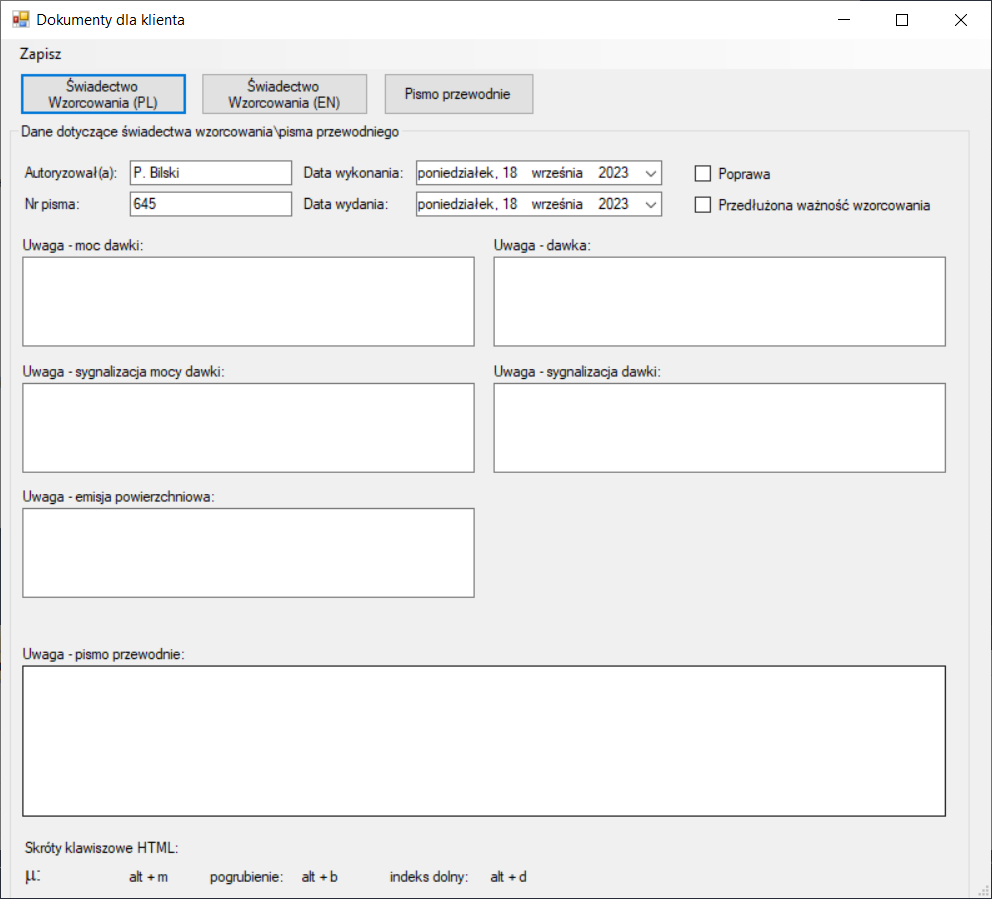
\includegraphics[width=\columnwidth]{obrazki/Wzorcowanie/menu_swiadectwo.png}
		\caption{Menu główne przygotowania i wydruku dokumentów.}
		\label{menuSwiadectwo}
	\end{figure}

	Główną część okna zajmują pola, w których możemy zamieścić uwagi do poszczególnych wyników wzorcowań albo do pisma przewodniego:
	\begin{itemize}
		\item \textbf{Uwaga - moc dawki} - pole do zamieszczenia uwagi, która umieszczona będzie na Świadectwie Wzorcowania w części dotyczącej wzorcowania w zakresie mocy dawki
		\item \textbf{Uwaga - dawka} - pole do zamieszczenia uwagi, która umieszczona będzie na Świadectwie Wzorcowania w części dotyczącej wzorcowania w zakresie dawki
		\item \textbf{Uwaga - sygnalizacja mocy dawki} - pole do zamieszczenia uwagi, która umieszczona będzie na Świadectwie Wzorcowania w części dotyczącej wzorcowania w zakresie sygnalizacji mocy dawki
		\item \textbf{Uwaga - sygnalizacja dawki} - pole do zamieszczenia uwagi, która umieszczona będzie na Świadectwie Wzorcowania w części dotyczącej wzorcowania w zakresie sygnalizacji dawki
		\item \textbf{Uwaga - emisja powierzchniowa} - pole do zamieszczenia uwagi, która umieszczona będzie na Świadectwie Wzorcowania w części dotyczącej wzorcowania w zakresie emisji powierzchniowej
		\item \textbf{Uwaga - pismo przewodnie} - pole do zamieszczenia uwagi, która umieszczona będzie na piśmie przewodnim
	\end{itemize}

	Na dole strony znajdują się skróty klawiszowe, których można użyć do wstawiania wybranych symboli, albo do formatowania tekstu:
	\begin{itemize}
		\item\textit{alt + m} - wstawia znacznik \textbf{\&mu;} oznaczający  $\mu$;
		\item\textit{alt + t} - wstawia znacznik \textbf{\&nbsp;} oznaczający twardą spację;
		\item\textit{alt + b} - wstawia \textbf{$<$b$>$$<$/b$>$} - tekst umieszczony w środku będzie pogrubiony (można najpierw użyć skrótu, w którym umieści się tekst, lub zaznaczyć wybrany fragment i wtedy użyć kombinacji klawiszy)
		\item\textit{alt + p} - wstawia \textbf{$<$br$>$} oznaczające przejście do kolejnej linii
		\item\textit{alt + d} - wstawia \textbf{$<$sub$>$$<$/sub$>$} - tekst umieszczony w środku będzie potraktowany jako indeks dolny (można najpierw użyć skrótu, w którym umieści się tekst, lub zaznaczyć wybrany fragment i wtedy użyć kombinacji klawiszy)
		\item\textit{alt + g} - wstawia \textbf{$<$sup$>$$<$/sup$>$} - tekst umieszczony w środku będzie potraktowany jako indeks górny (można najpierw użyć skrótu, w którym umieści się tekst, lub zaznaczyć wybrany fragment i wtedy użyć kombinacji klawiszy)
	\end{itemize}

	\textbf{TIP:} We wszystkich uwagach można stosować dowolne znaczniki języka HTML.

	W górnym menu okna znajduje się przycisk \textbf{"Zapisz"}, który umożliwia zapisanie wprowadzonych zmian.
	
	Przyciski \textbf{"Świadectwo Wzorcowania (PL)"}, \textbf{Świadectwo Wzorcowania (EN)} i \textbf{"Pismo przewodnie"} generują odpowiednio świadectwo wzorcowania w języku polskim, angielskim i pismo przewodnie.
	
	Jeżeli w celu utworzenie świadectwa wzorcowania w języku angielskim program będzie potrzebował tłumaczenia dodatkowych słów, to otwarte zostanie okno \textbf{"Tłumaczenie słowa"} (rys. \ref{tlumaczenie}).
	Program zapyta, co ma zrobić z nieznanym mu słowem podanym w pierwszym polu. Można wybrać opcję \textbf{"Nie tłumacz"}, wtedy na świadectwie słowo to pozostanie niezmienione lub opcję \textbf{"Przetłumacz na:"} i podać w polu obok żądane tłumaczenie. 
	
	\textbf{TIP:} Jeżeli jest to często powtarzające się słowo lub sformułowanie  np. \textit{radiometr, dawkomierz, nie dotyczy} można zaznaczając pole wyboru \textbf{"Zapamiętaj mój wybór"} na stałe dopisać je do słownika programu.

		
	\begin{figure}[htb]
		\centering
		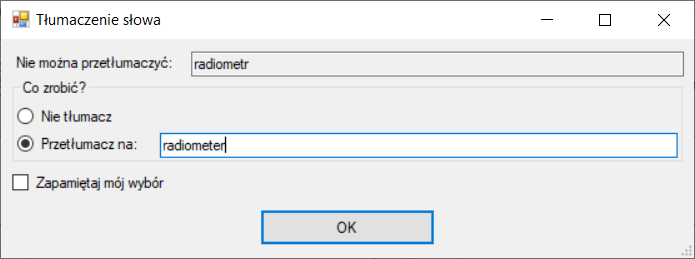
\includegraphics[width=\columnwidth]{obrazki/Wzorcowanie/tlumaczenie.png}
		\caption{Dodawanie brakujących słów do słownika.}
		\label{tlumaczenie}
	\end{figure}

	\textbf{TIP:} Należy pamiętać, że wszelkie uwagi w polach \textbf{"Uwaga - moc dawki"}, \textbf{"Uwaga - dawka"}, \textbf{"Uwaga - sygnalizacja mocy dawki"}, \textbf{"Uwaga - sygnalizacja dawki"}, \textbf{"Uwaga - emisja powierzchniowa"} powinny zostać napisane w języku docelowym, gdyż nie podlegają one tłumaczeniu, a są bezpośrednio wstawiane do świadectwa wzorcowania.